%%%%%%%%%%%%%%%%%%%%%%%%%%%%%%%%%%%%%%%%%%%%%%%%%%%%%%%%%%%%%%%%%%%%%
%% This is a (brief) model paper using the achemso class
%% The document class accepts keyval options, which should include
%% the target journal and optionally the manuscript type.
%%%%%%%%%%%%%%%%%%%%%%%%%%%%%%%%%%%%%%%%%%%%%%%%%%%%%%%%%%%%%%%%%%%%%
\documentclass[journal=jacsat,manuscript=article]{achemso}

%%%%%%%%%%%%%%%%%%%%%%%%%%%%%%%%%%%%%%%%%%%%%%%%%%%%%%%%%%%%%%%%%%%%%
%% Place any additional packages needed here.  Only include packages
%% which are essential, to avoid problems later. Do NOT use any
%% packages which require e-TeX (for example etoolbox): the e-TeX
%% extensions are not currently available on the ACS conversion
%% servers.
%%%%%%%%%%%%%%%%%%%%%%%%%%%%%%%%%%%%%%%%%%%%%%%%%%%%%%%%%%%%%%%%%%%%%
\usepackage[version=3]{mhchem} % Formula subscripts using \ce{}
\usepackage{color}  % remove this package once you are done
\usepackage{multirow}
%%%%%%%%%%%%%%%%%%%%%%%%%%%%%%%%%%%%%%%%%%%%%%%%%%%%%%%%%%%%%%%%%%%%%
%% If issues arise when submitting your manuscript, you may want to
%% un-comment the next line.  This provides information on the
%% version of every file you have used.
%%%%%%%%%%%%%%%%%%%%%%%%%%%%%%%%%%%%%%%%%%%%%%%%%%%%%%%%%%%%%%%%%%%%%
%%\listfiles

%%%%%%%%%%%%%%%%%%%%%%%%%%%%%%%%%%%%%%%%%%%%%%%%%%%%%%%%%%%%%%%%%%%%%
%% Place any additional macros here.  Please use \newcommand* where
%% possible, and avoid layout-changing macros (which are not used
%% when typesetting).
%%%%%%%%%%%%%%%%%%%%%%%%%%%%%%%%%%%%%%%%%%%%%%%%%%%%%%%%%%%%%%%%%%%%%
\newcommand*\mycommand[1]{\texttt{\emph{#1}}}
%%%%%%%%%%%%%%%%%%%%%%%%%%%%%%%%%%%%%%%%%%%%%%%%%%%%%%%%%%%%%%%%%%%%%
%% Meta-data block
%% ---------------
%% Each author should be given as a separate \author command.
%%
%% Corresponding authors should have an e-mail given after the author
%% name as an \email command. Phone and fax numbers can be given
%% using \phone and \fax, respectively; this information is optional.
%%
%% The affiliation of authors is given after the authors; each
%% \affiliation command applies to all preceding authors not already
%% assigned an affiliation.
%%t
%% The affiliation takes an option argument for the short name.  This
%% will typically be something like "University of Somewhere".
%%
%% The \altaffiliation macro should be used for new address, etc.
%% On the other hand, \alsoaffiliation is used on a per author basis
%% when authors are associated with multiple institutions.
%%%%%%%%%%%%%%%%%%%%%%%%%%%%%%%%%%%%%%%%%%%%%%%%%%%%%%%%%%%%%%%%%%%%%
\author{Ruchi Lohia}
%\altaffiliation{A shared footnote}
\author{Reza Salari}
%\altaffiliation{Current address: Some other place, Othert\"own,
%Germany}
\author{Grace Brannigan}
\email{grace.brannigan@rutgers.edu(GB)}
\affiliation[Rutgers University]
{Center for Computational and Integrative Biology, Rutgers University, Camden, NJ, USA}
\alsoaffiliation[Rutgers University]
{ Department of Physics, Rutgers University, Camden, NJ, USA}

%%%%%%%%%%%%%%%%%%%%%%%%%%%%%%%%%%%%%%%%%%%%%%%%%%%%%%%%%%%%%%%%%%%%%
%% The document title should be given as usual. Some journals require
%% a running title from the author: this should be supplied as an
%% optional argument to \title.
%%%%%%%%%%%%%%%%%%%%%%%%%%%%%%%%%%%%%%%%%%%%%%%%%%%%%%%%%%%%%%%%%%%%%
\title[An \textsf{achemso} demo]
  {Sequence specificity despite intrinsic disorder: how a disease-associated  Val/Met polymorphism shifts tertiary interactions in a long disordered protein}

%%%%%%%%%%%%%%%%%%%%%%%%%%%%%%%%%%%%%%%%%%%%%%%%%%%%%%%%%%%%%%%%%%%%%
%% Some journals require a list of abbreviations or keywords to be
%% supplied. These should be set up here, and will be printed after
%% the title and author information, if needed.
%%%%%%%%%%%%%%%%%%%%%%%%%%%%%%%%%%%%%%%%%%%%%%%%%%%%%%%%%%%%%%%%%%%%%
\abbreviations{IR,NMR,UV}
\keywords{American Chemical Society, \LaTeX}
\usepackage{makecell}
\renewcommand{\thepage}{S\arabic{page}}  
\renewcommand{\thesection}{S\arabic{section}}   
\renewcommand{\thetable}{S\arabic{table}}   
\renewcommand{\figurename}{}
\renewcommand{\thefigure}{Fig S\arabic{figure}}

\begin{document}

\clearpage


\begin{figure}[!ht]
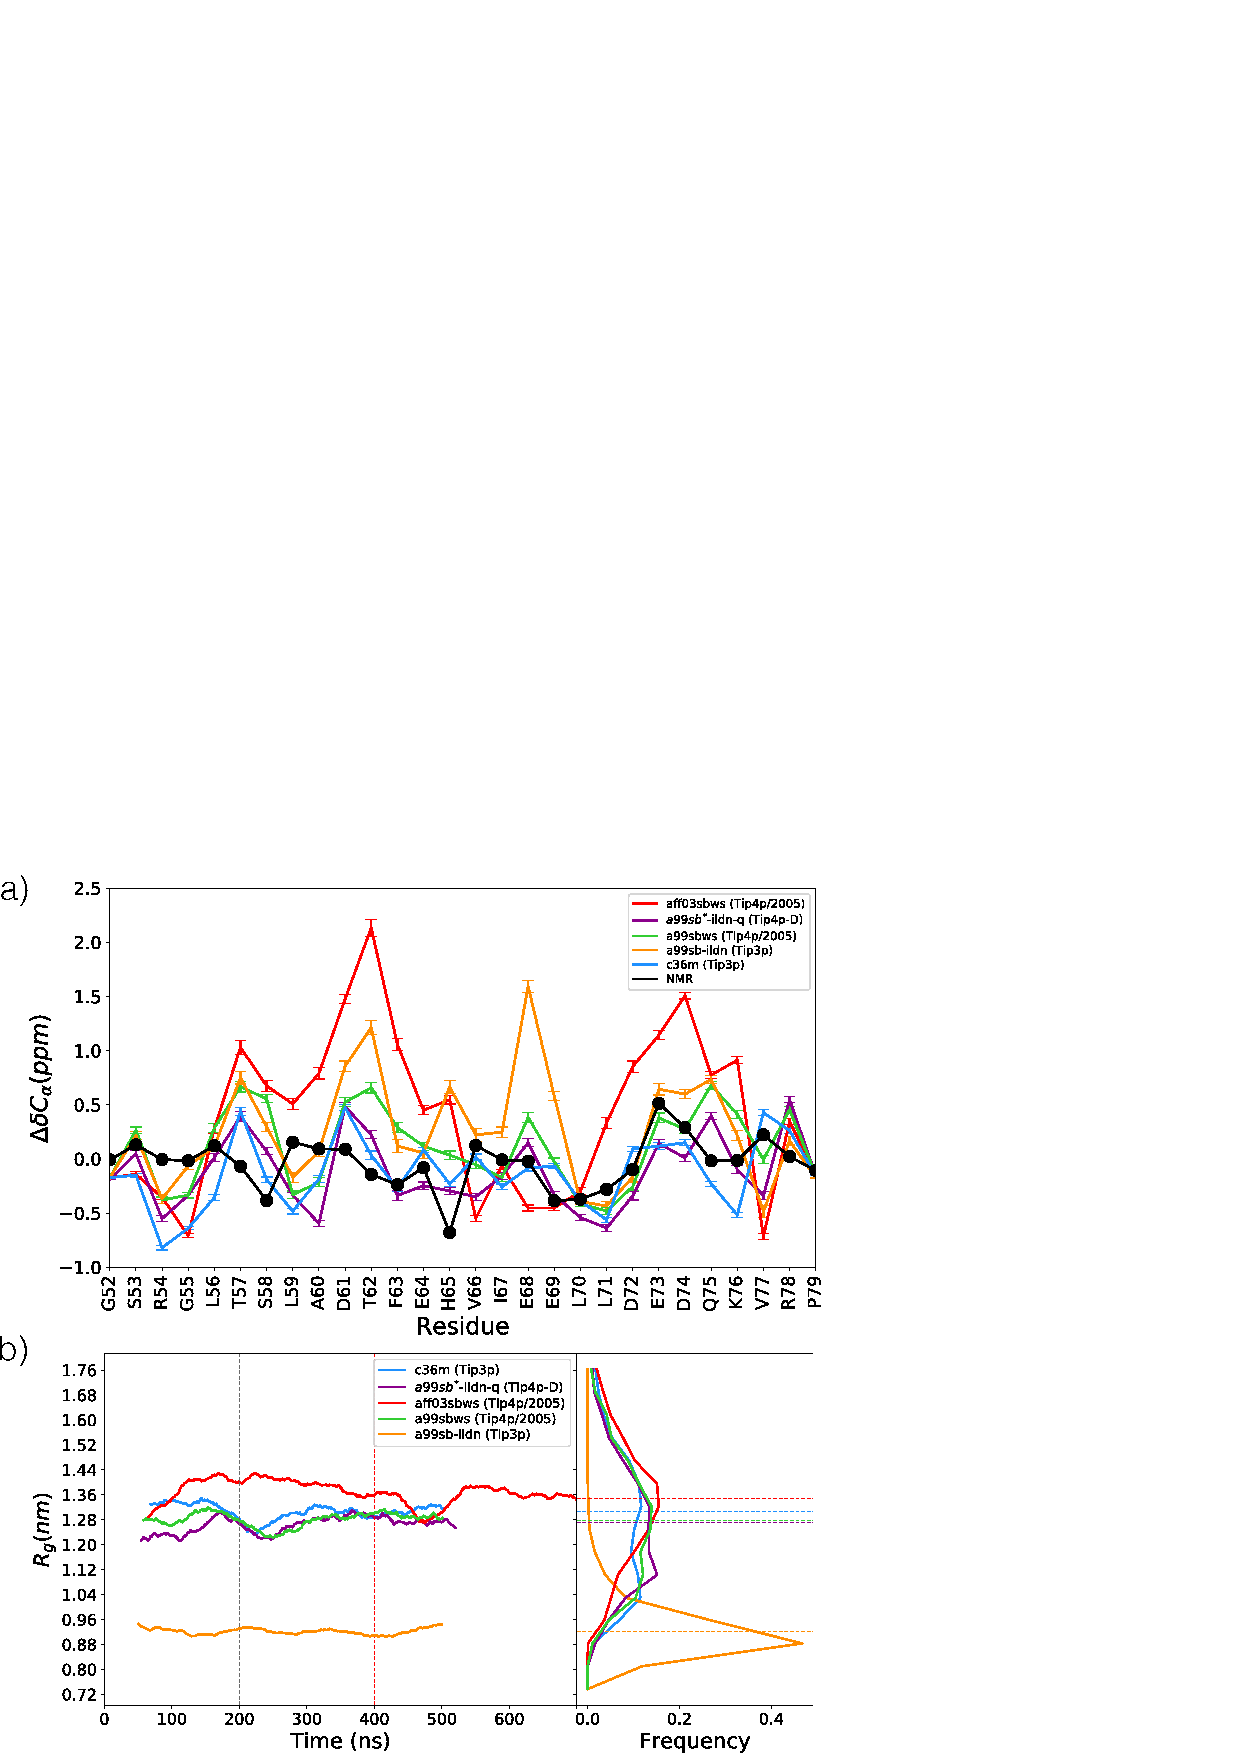
\includegraphics[scale=0.5,width=0.9\textwidth,trim={0 0cm 0 0cm},clip]{../figures/S1.pdf}
\caption{{\bf Force field comparison.} We ran 500ns of T-REMD simulations of a 30 residue fragment of the V66 prodomain with several commonly used force field and water model combinations. The first 200ns of data was discarded as equilibration. (a) Comparison of calculated C\textsubscript{$\alpha$} chemical shifts from MD ensembles at 280K for Amber99sb*-ildn-q ~\cite {Lindorff-Larsen2010a, Hornak2006a} with Tip4p-D ~\cite {Piana2015} (RMSD 0.36 ppm),  Amber99sbws ~\cite {Lindorff-Larsen2010a, Best2014} (RMSD 0.42 ppm), Amberff03sbws  ~\cite {Best2009, Best2014} (RMSD 0.73 ppm), Amber99sb-ildn with Tip3P ~\cite {Jorgensen1981} (RMSD 0.65 ppm), calculated using SPARTA+ ~\cite{Shen2010} and NMR C\textsubscript{$\alpha$} chemical shifts (black line) from Ref.~\citenum{Anastasia2013} at 280K. (b) R\textsubscript{g} distribution for each force field. Tip3P generates very collapsed ensembles and the remaining three force field generates similar R\textsubscript{g} distribution. The $\langle R\textsubscript{g} \rangle$ is shown with vertical lines.}
\label{S1} 
\end{figure}


 \begin{figure}[!ht]
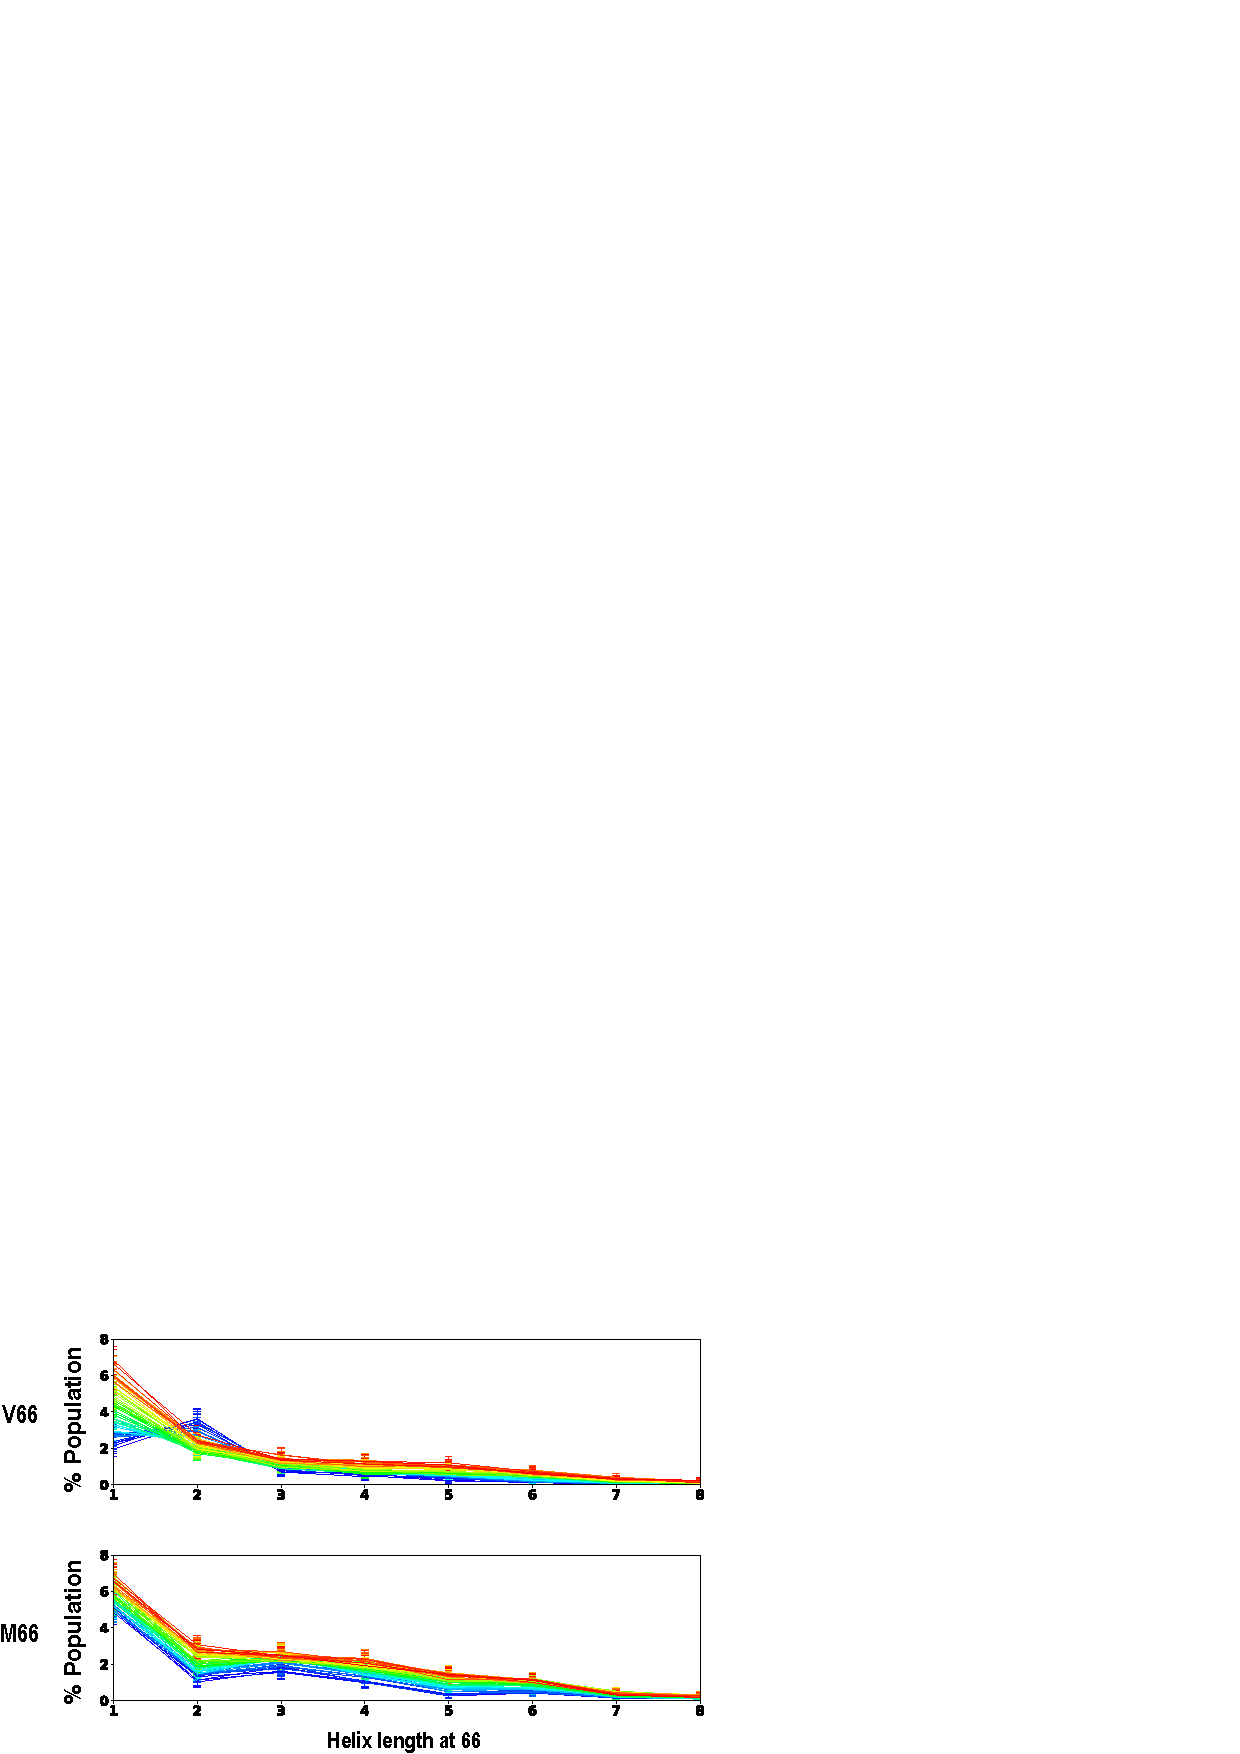
\includegraphics[scale=0.5,width=\textwidth,trim={0 0cm 0 0cm},clip]{../figures/S2.pdf}
\caption{{\bf Comparison of MD and NMR observables.} C\textsubscript{$\alpha$} (top) and C\textsubscript{$\beta$} (bottom) chemical shifts from NMR at 280K (black lines)~\cite{Anastasia2013} and MD at 300K (blue lines), calculated using SPARTA+ ~\cite{Shen2010} for M66 sequence. Chemical shifts outside the range of 0.5 ppm from NMR chemical shifts are shaded grey.}
\label{S2} 
\end{figure}

\begin{figure}[!ht]
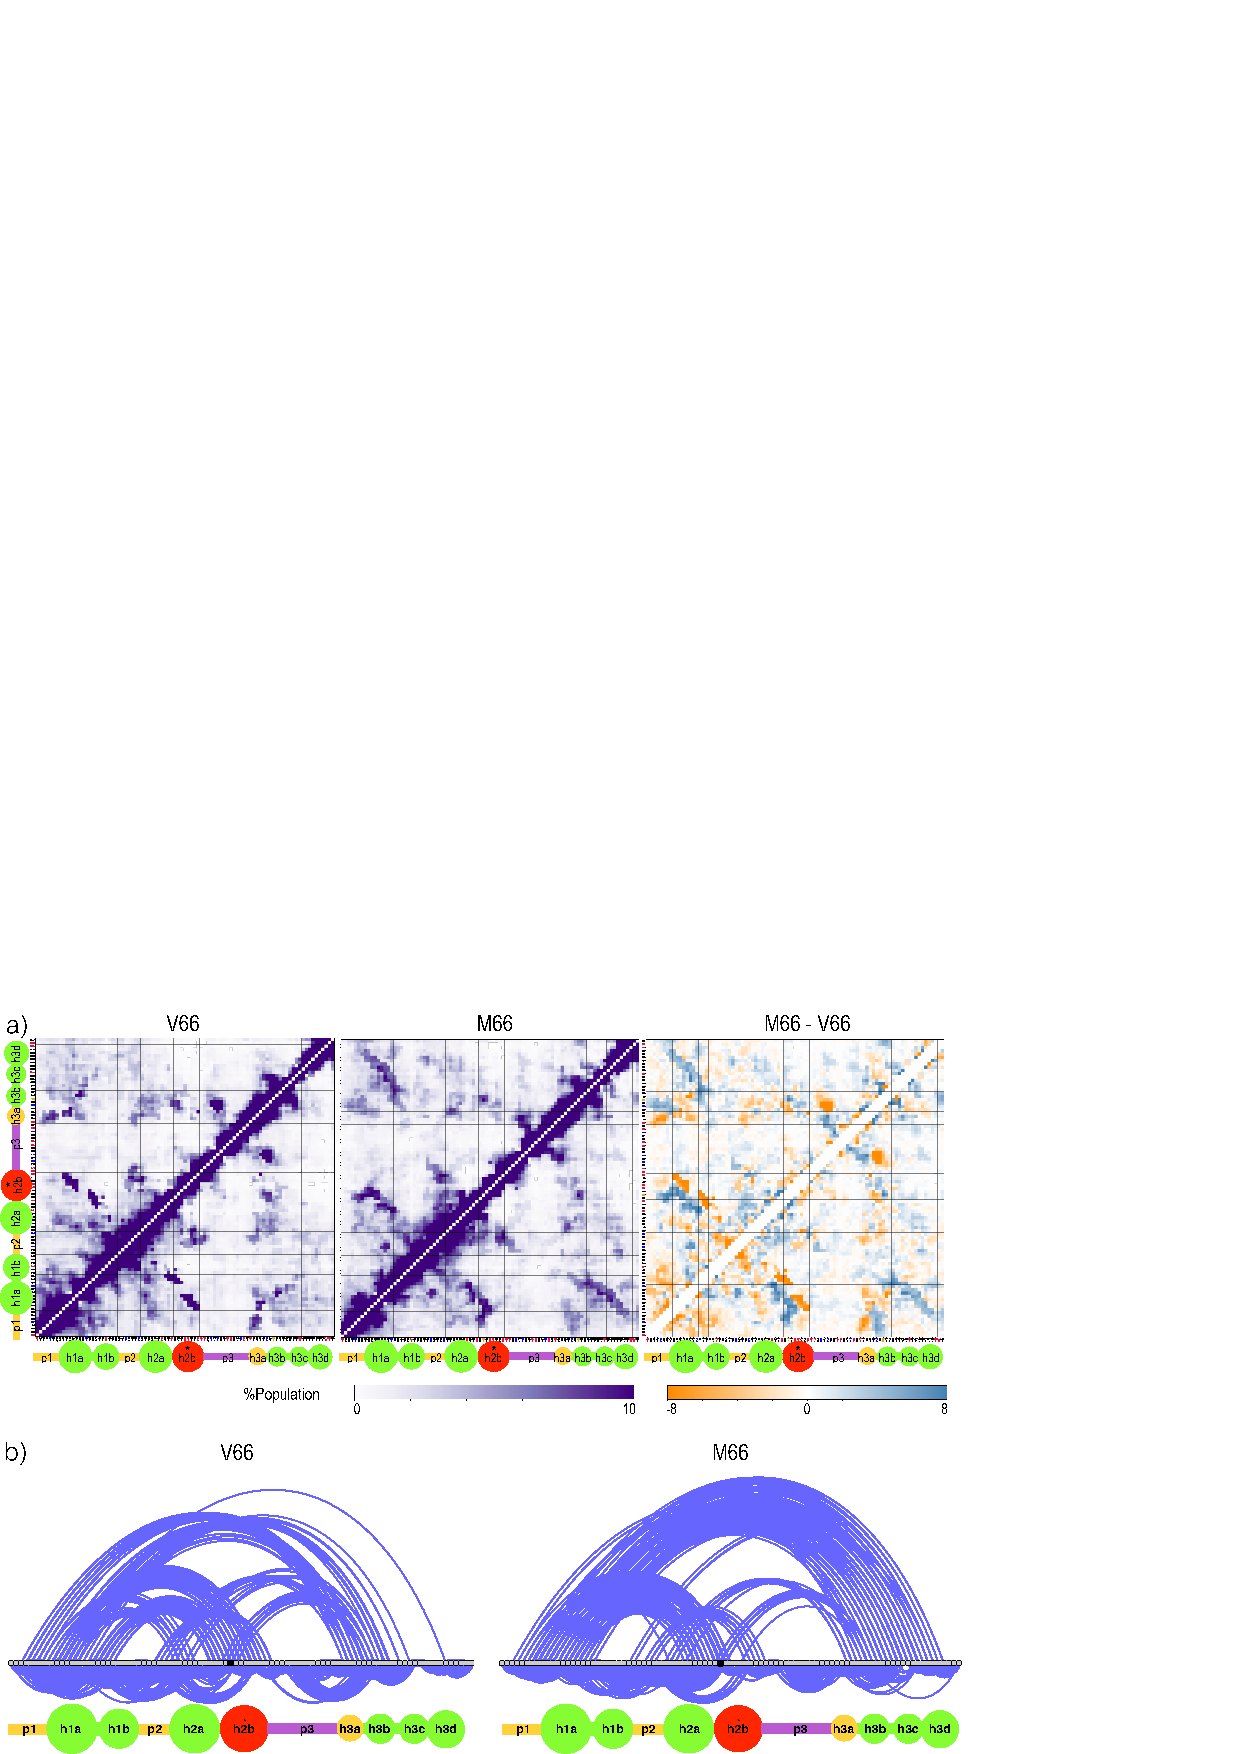
\includegraphics[scale=0.5,width=0.9\textwidth,trim={0 0cm 0 0cm},clip]{../figures/S3.pdf}
\caption{{\bf Scaling behavior of each identified domain.} Ensemble averaged interchain distance profiles for each domain in V66 sequence. Theoretical polymer scaling limits are shown with grey lines (prefactor A = 0.55 nm), while Flory exponents for each curve are given in Table~\ref{t1}. }
\label{S3} 
\end{figure}

\begin{table}[ht]
\caption{Flory exponent ($\nu$) and prefactor (A) for each proregion domain, calculated from MD trajectories. Errors represent fit error of $\langle R_{|i-j|}\rangle$ vs  $An^{\nu}$, weighted by each point's standard deviation.}
\label{t1}
\begin{tabular}{|c|c|c|c|c|}
\hline
domain & A (V66)  & $\nu$ (V66) & A (M66)  & $\nu$ (M66)\\          
\hline
p1 &  0.53 $\pm{ 0.16}$ & 0.58 $\pm{ 0.24}$ &  0.52 $\pm{0.15}$ & 0.60 $\pm{0.23}$ \\
\hline
h1a &  0.53 $\pm{ 0.16}$ & 0.59 $\pm{ 0.25}$ &  0.53 $\pm{0.16}$ & 0.60 $\pm{0.24}$ \\
\hline
h1b & 0.61  $\pm{0.24 }$ &0.44  $\pm{0.40 }$ &  0.60 $\pm{0.26}$ & 0.44 $\pm{0.41}$ \\
\hline
p2 & 0.56  $\pm{0.22 }$ &0.50  $\pm{0.34 }$ &  0.59 $\pm{0.18}$ & 0.51 $\pm{0.29}$ \\
\hline
h2a &  0.56 $\pm{ 0.17}$ & 0.50 $\pm{ 0.22}$ &  0.57 $\pm{0.17}$ & 0.48 $\pm{0.23}$ \\
\hline
h2b &  0.64 $\pm{ 0.14}$ & 0.51 $\pm{ 0.18}$ &  0.60 $\pm{0.15}$ & 0.56 $\pm{0.20}$ \\
\hline
p3 &  0.49 $\pm{ 0.09}$ & 0.63 $\pm{ 0.10}$ &  0.50 $\pm{0.09}$ & 0.62 $\pm{0.10}$ \\
\hline
h3b &  0.56 $\pm{ 0.32}$ & 0.55 $\pm{ 0.62}$ &  0.55 $\pm{0.28}$ & 0.60 $\pm{0.57}$ \\
\hline
h3c &  0.52 $\pm{ 0.13}$ & 0.75 $\pm{ 0.29}$ &  0.52 $\pm{0.14}$ & 0.74 $\pm{0.31}$ \\
\hline
h3d & 0.58  $\pm{0.18 }$ &0.52  $\pm{0.27 }$ &  0.59 $\pm{0.19}$ & 0.49 $\pm{0.28}$ \\
\hline
\end{tabular}

\end{table}

 \begin{figure}[!ht]
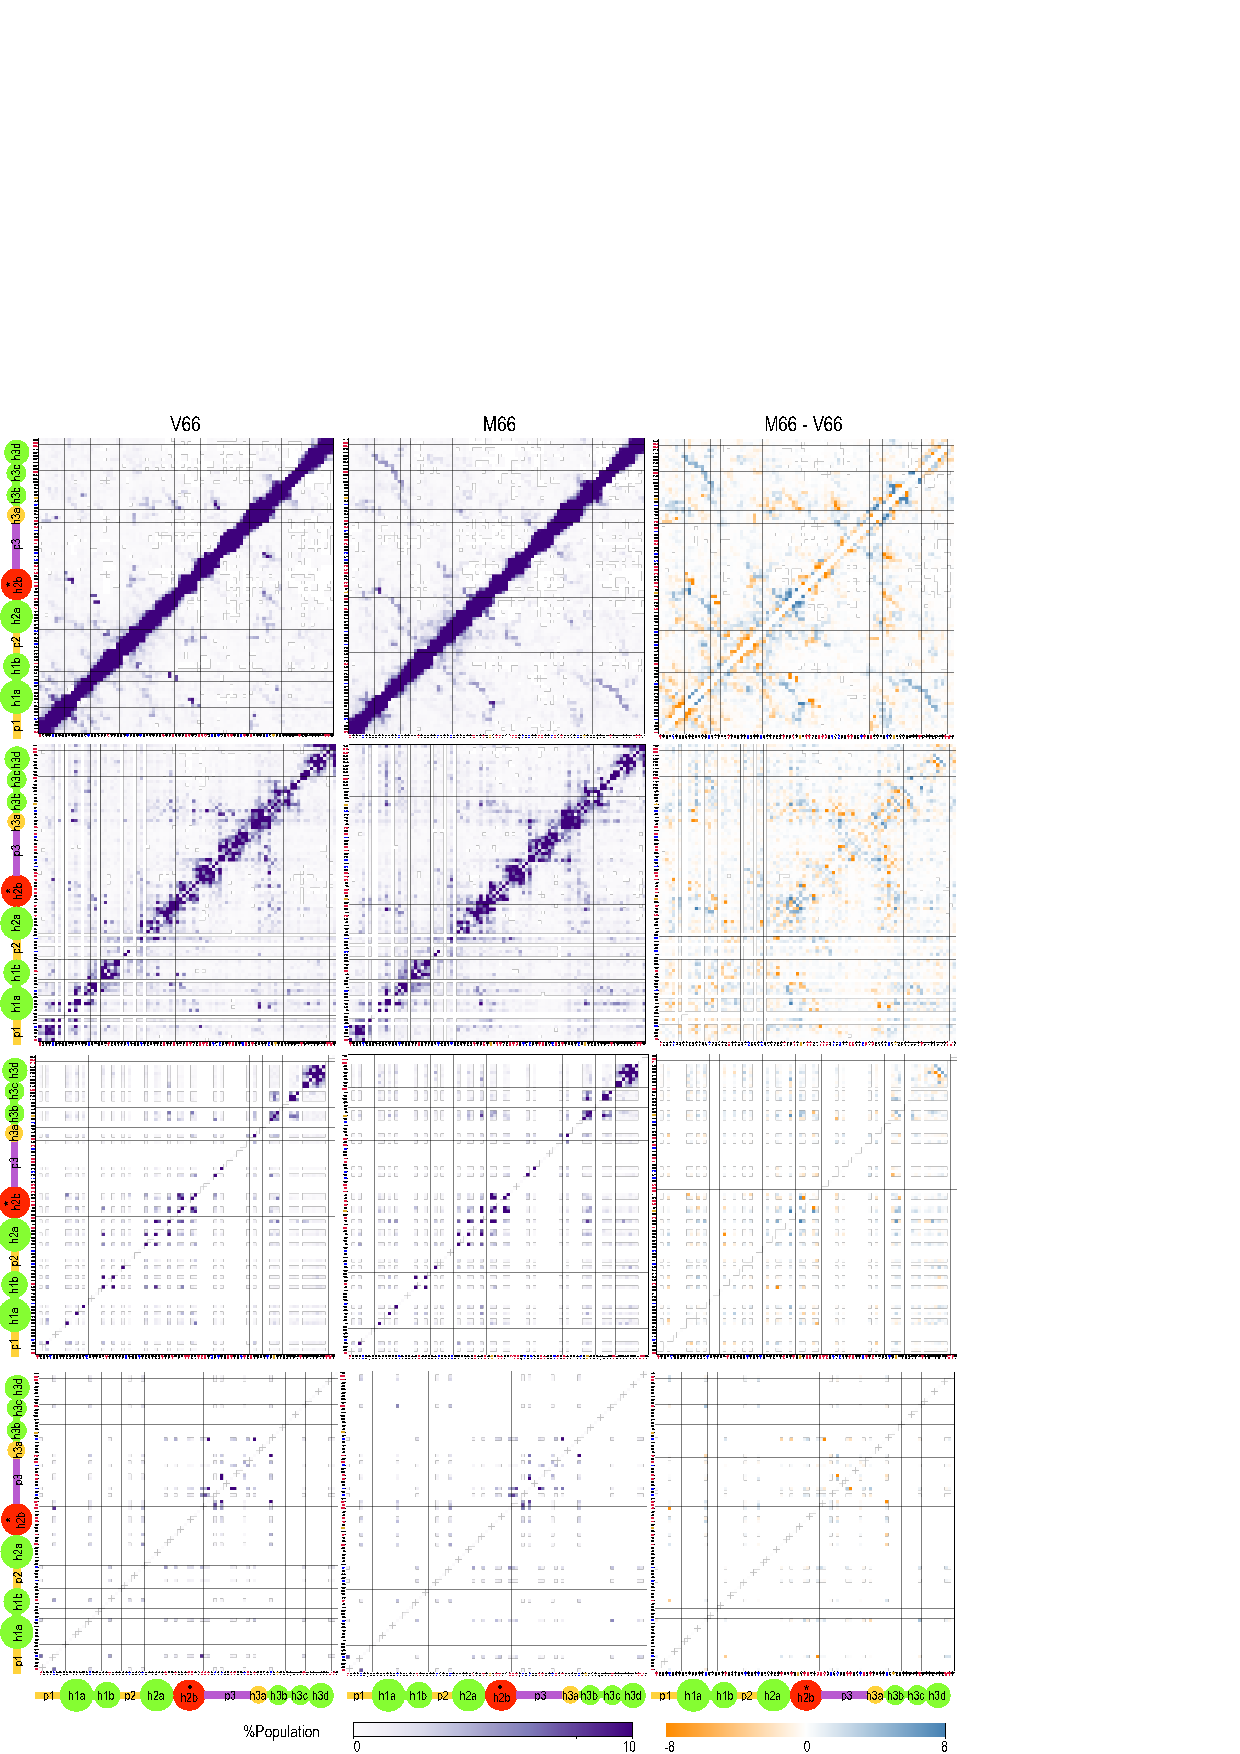
\includegraphics[scale=0.5,width=\textwidth,trim={0 0cm 0 0cm},clip]{../figures/S4.pdf}
\caption{{\bf Effect of perturbing monomer properties on freely-jointed, self-avoiding heteropolymer} Contact probability maps from MC simulations, analogous to those in Figure 3 of the main text, in which the monomer with properties of linker domain p3 is swapped with every other monomer on the chain, with the new location represented by the purple square in the graph annotation.  As the p3 bead is shifted along the chain, p3 and p1 consistently bound a white ``forbidden'' region that has little interaction with the rest of the protein. }
\label{S4} 
\end{figure}

 \begin{figure}[!ht]
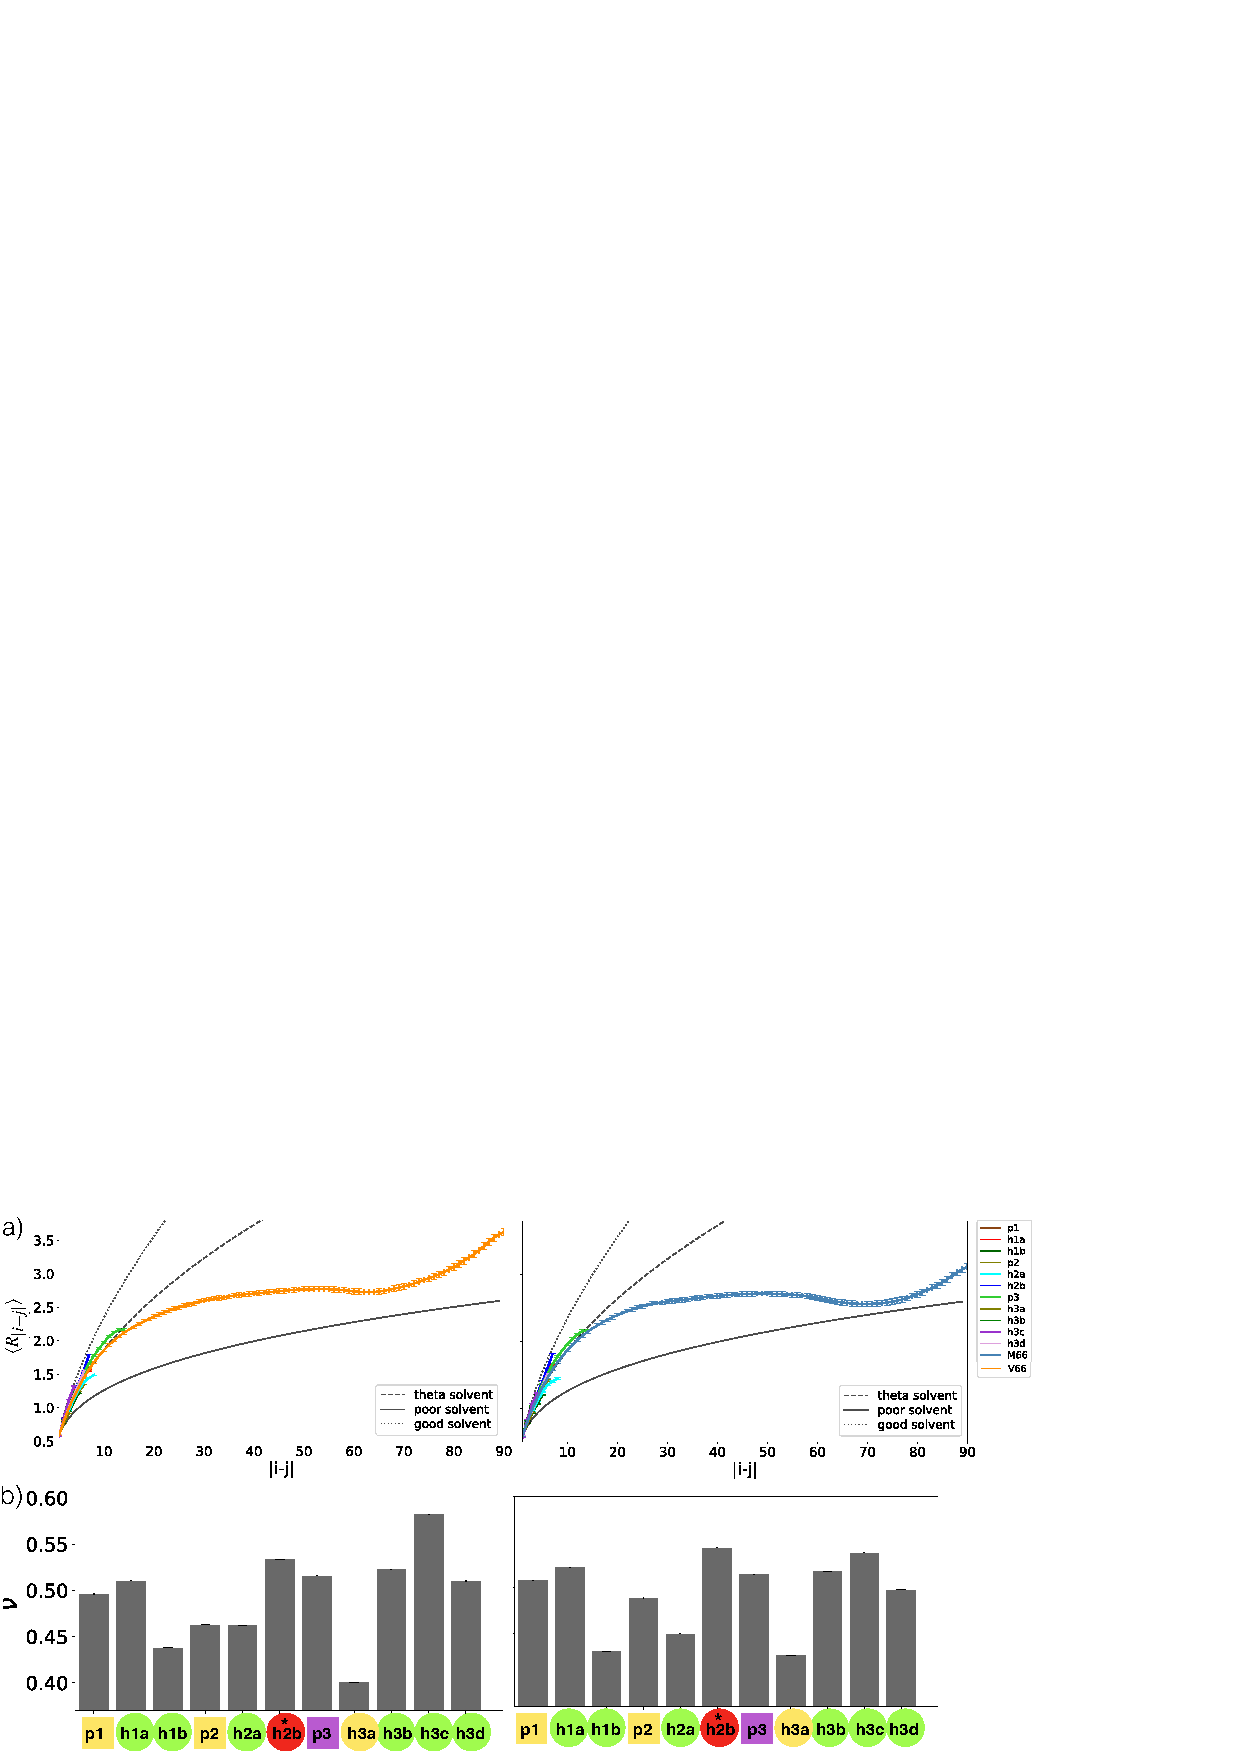
\includegraphics[scale=0.5,width=\textwidth,trim={0 0cm 0 0cm},clip]{../figures/S5.pdf}
\caption{{\bf Residue level contacts for the entire prodomain.} Contact probability between every residue pair for V66 (left) and M66 (right). A linear network of transient tertiary contacts is also shown (top) for each form. Two residue pairs are in contact if the distance between C\textsubscript{$\alpha$}-C\textsubscript{$\alpha$} atoms between the two residues are 0.8nm or less. The contact networks were build using Cytoscape ~\cite {Ahlstrom2013} with a linear representation of residues. Each protein residue comprises a node in the network, with interactions between residues represented as edges. The strength of individual interactions can be interpreted by the thickness of the edge line on the network diagram. If the separation between residues forming the contact is more than 3, its edge is drawn above the node; otherwise, the edge is drawn at the bottom of the node. To focus on significant interactions, interactions showing more than 4\% persistence were considered in network visualization.}
\label{S5} 
\end{figure}

\begin{figure}[!ht]
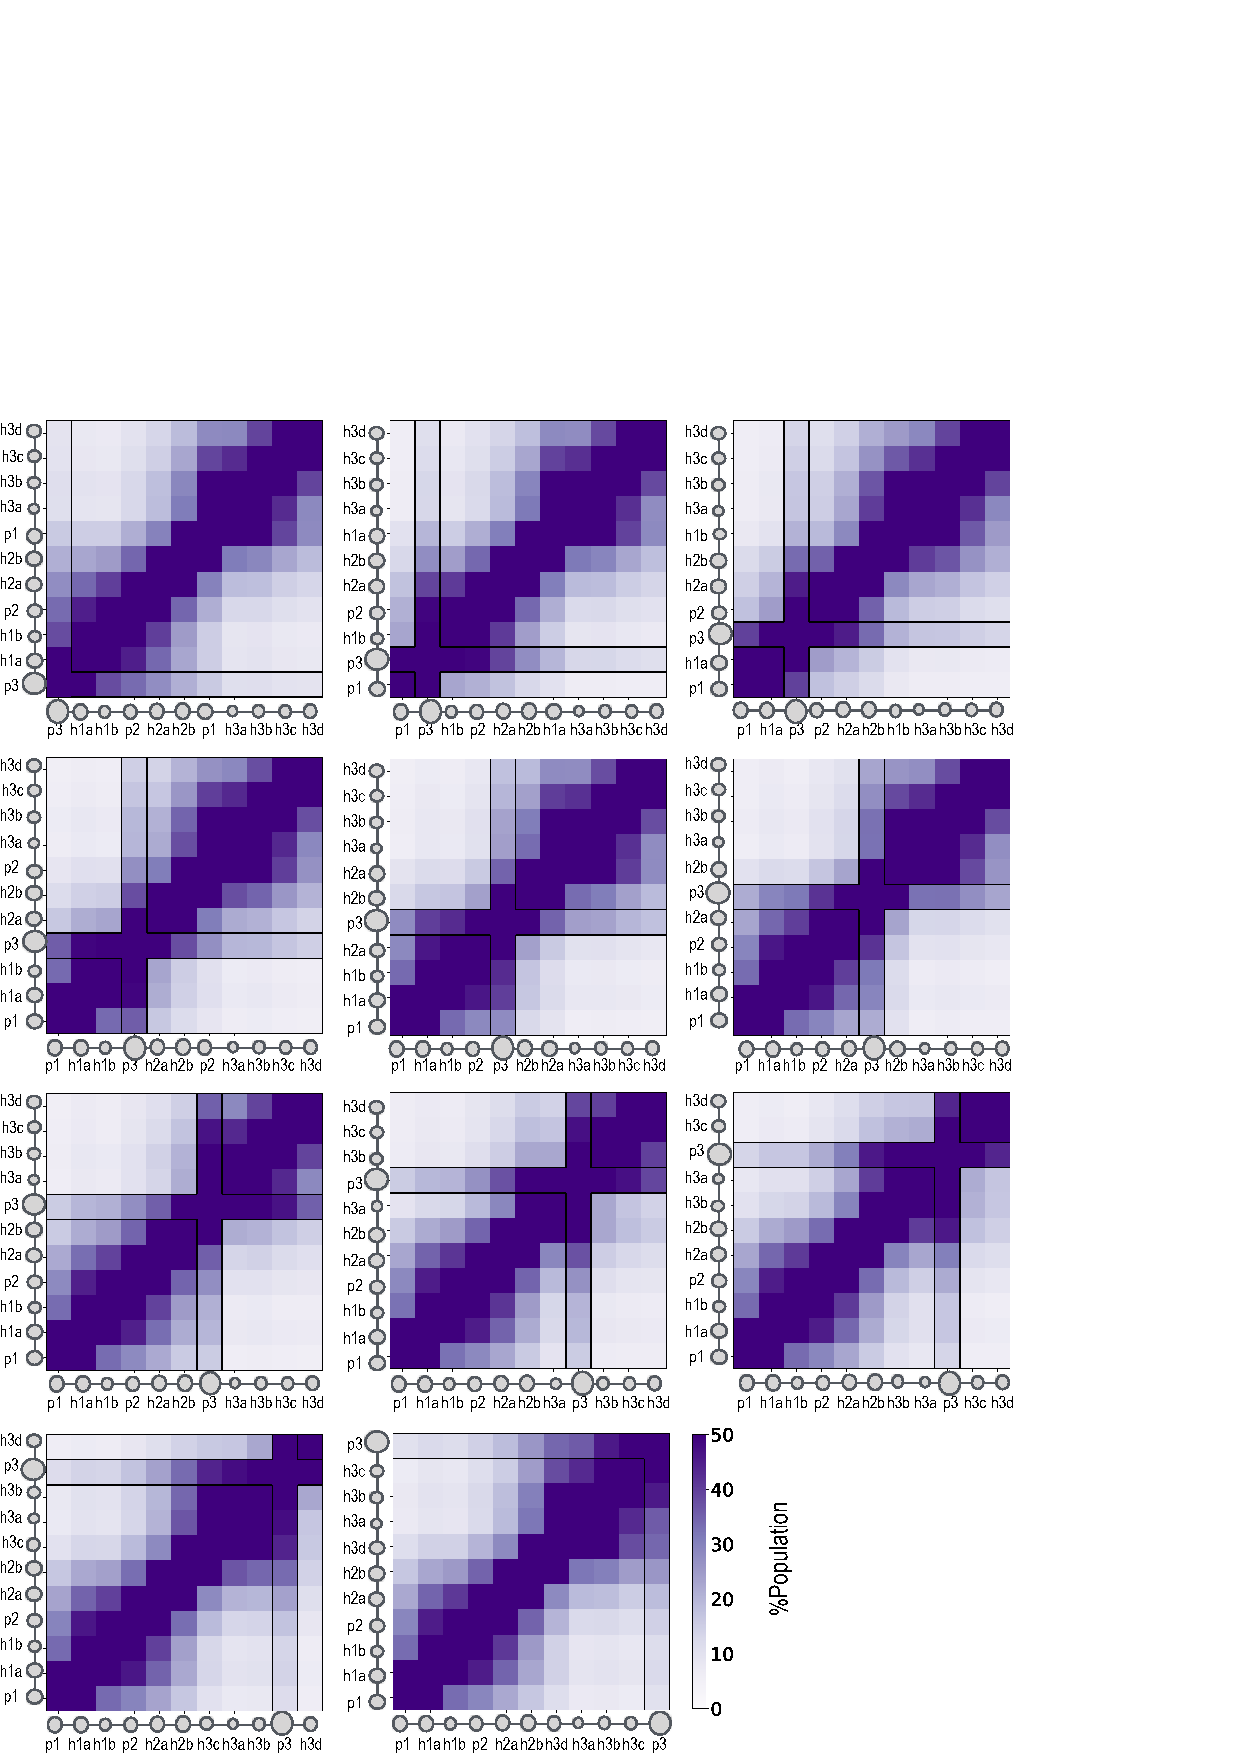
\includegraphics[scale=0.5,width=0.9\textwidth,trim={0 0cm 0 0cm},clip]{../figures/S6.pdf}
\caption{{\bf Effects of temperature and Val66Met mutation on helix propensity around residue 66.} Frequency of helix of a given length at residue 66 in V66 (top) and M66 (bottom) in the temperature range of 300K to 385 K. With the increase in temperature the color transitions from cooler (blue) to hotter (red).  It is entropically unfavorable for V66 and its neighboring residue to be simultaneously in the helical region of the Ramachandran map, as indicated by the decreasing helical propensity with increasing temperature.  For longer helices, the trend will depend more on the additional side-chains in the helix, and the trend with temperature is reversed, but it remains weaker than the analogous trend for the M66 sequence.  Errors represent standard error of a Bernoulli trial with n number of samples, where n is the product of total number unique replicas forming the helix of given length at residue 66 at a given temperature and average number of roundtrips per replica, 17.}
\label{S6} 
\end{figure}

\begin{figure}[!ht]
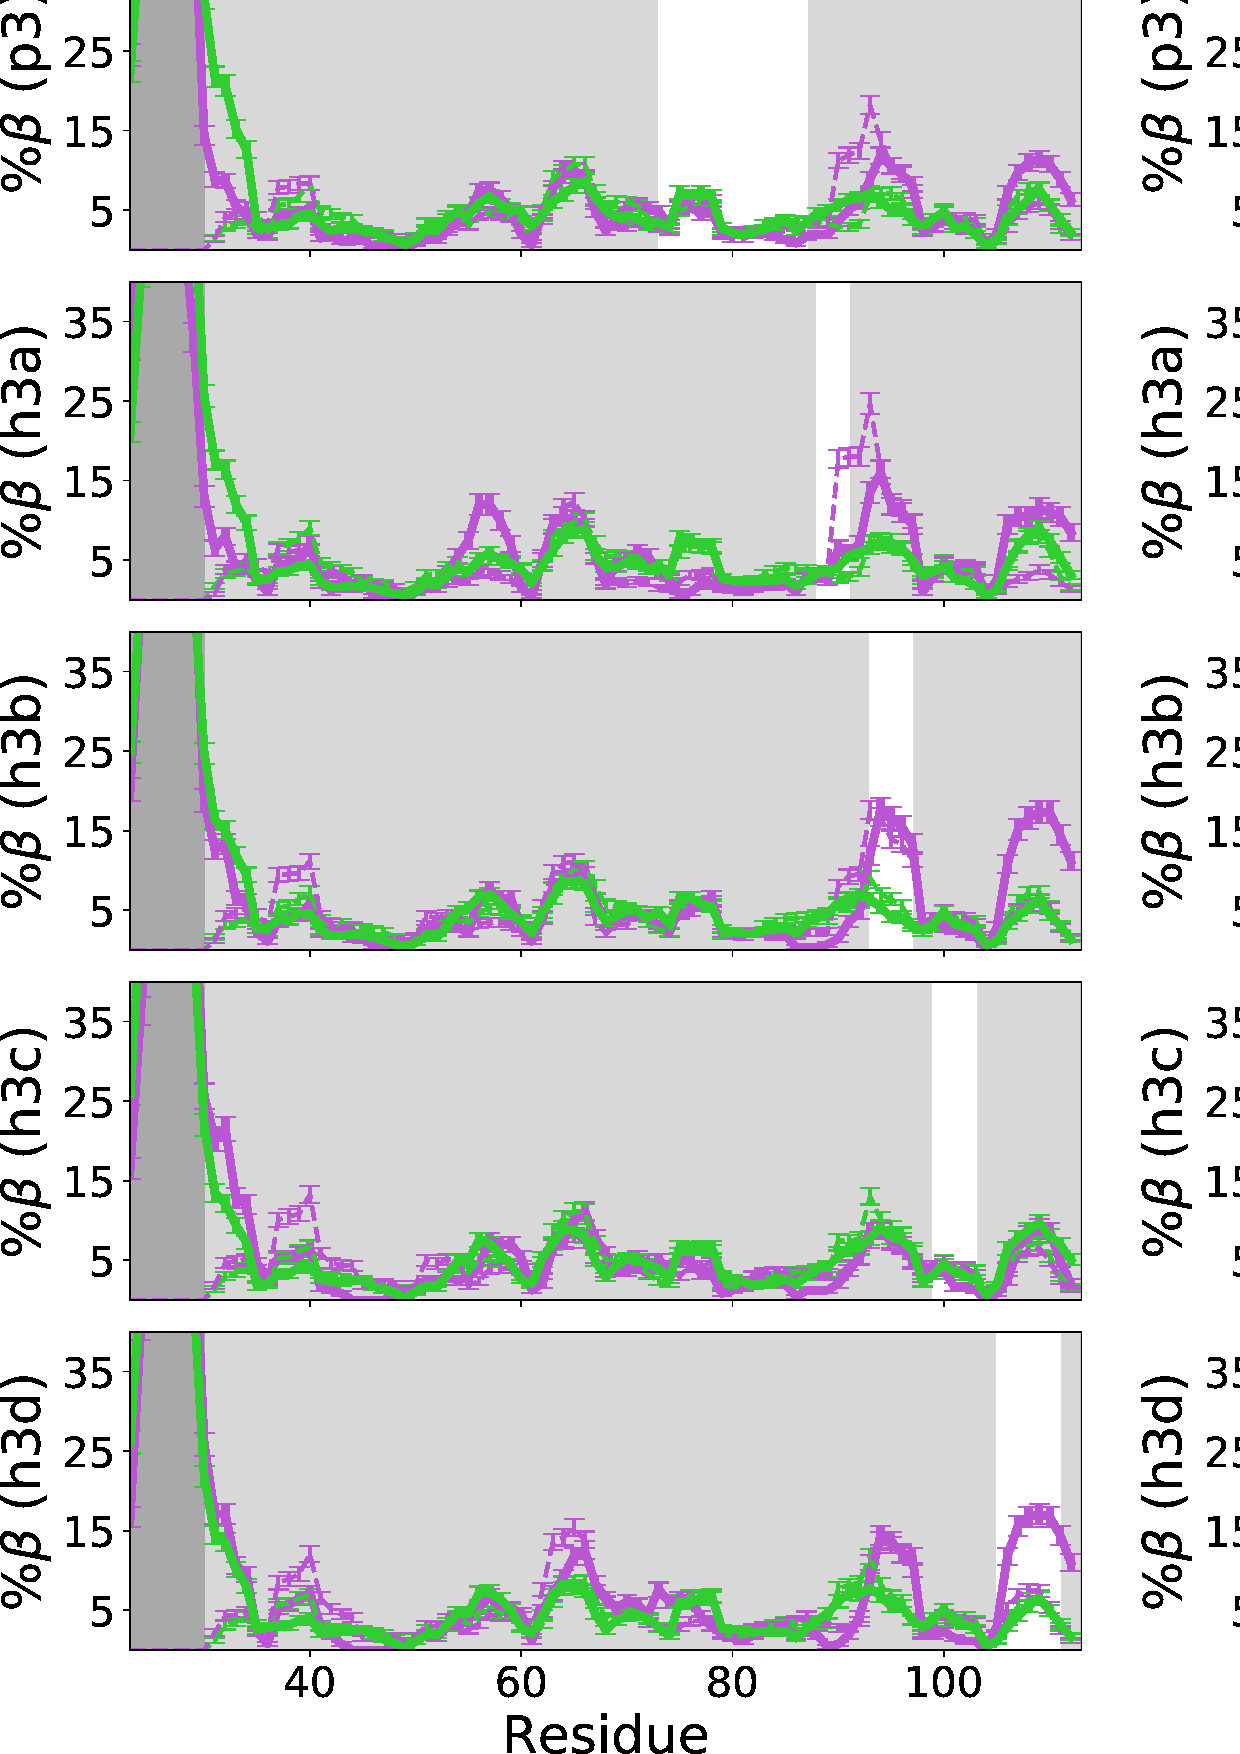
\includegraphics[scale=0.5,width=0.9\textwidth,trim={0 0cm 0 0cm},clip]{../figures/S7.pdf}
\caption{{\bf Number of round trip completed by each replica.} Both V66 and M66 complete a minimum 5 roundtrips for each replica and an average of 17 round-tips per replica over the course of 76.8 $\mu$s (1.2 $\mu$s $\times$64) of simulations.}
\label{S7} 
\end{figure}


\clearpage
\bibliography{Jacs_ref}

\end{document}

